% Chapter 1

\chapter{Conclusions} % Main chapter title
\label{Chapter6} % For referencing the chapter elsewhere, use \ref{Chapter1} 

\section{Summary}

We have assimilated observations of $H_s, T_{m01} \text{ and } T_{m02}$ into Fugro's wave forecasts in the GoM region. To do this, we made use of the update step from the ETKF method to correct an entire 7-day forecast run in one go. This differs from conventional ETKF implementations, in which simultaneous observations are assimilated together and then the forecast model is used to step the state forward to the next observation time.

Investigating the background errors, we found that the ensemble variance in $H_s$ is a strong function of $H_s$ itself, and it peaks just before the peak in $H_s$. A similar relationship was found for $T_{m01}$. We saw that the forecast error covariances are often strongest near the buoy location, and longer distance covariances can arise physically due to winds and travelling waves and also spuriously due to sampling error.

We found that observation errors are a strong linear function of the variable being observed, particularly in $H_s$. This motivated us to set the observation error standard deviation in the DA system to a linear scale of the observations. Since the scaling factor for the periods was small, we implemented a constant minimum error threshold for these variables to ensure that the error would not become too small and negatively impact DA performance.

We compared the results of assimilating $H_s$ alone ($H_s$ DA) to assimilating all three variables (all vars DA), and found that both approaches, but particularly all vars DA, produced somewhat unrealistic increments with large changes to the state far away from the observation location. Comparing our results to \citet{Houghton2023} (figure \ref{fig:houghton2022fig3} and figure \ref{fig:hsinc}), we see that their LETKF method produced more realistic increments, which captured the flow dependency of the background covariances while keeping the effects of the observations confined to the vicinity of the observation location.

We found reductions in RMSE of up to 50\% in both variables, which extended up to 0.5 days beyond the end of the asssimilation window in the case of $H_s$ DA, and 1.5 days beyond in the case all vars DA. Both cases produced very similar RMSE reductions during the assimilation window, and all vars DA had consistently smaller errors than $H_s$ DA at >1 day after the end of assimilation. At 2-3 days after assimilation, both DA runs had larger errors than the no DA case. %(and we were unable to find an explanation for this).

These improvements in RMSE are less consistent and slightly shorter lived than those obtained in \cite{Houghton2022,Houghton2023} (figures \ref{fig:houghton2022fig3}, \ref{fig:houghton2023fig6}). This reflects the two major limitations identified in section \ref{sec:prevwork}, namely the limited number of observations available to us and the fact that we do not have access to the forecast model, which means that we must update an entire forecast run in one update step and not use cycling. Our results agree with \cite{Houghton2022} in that assimilating multiple variables (spectral DA) performed better than assimilating wave height alone in most cases. One difference between the results of that study and this is that \cite{Houghton2022} found $H_s$ DA and spectral DA to be virtually identical in predicting $H_s$, while spectral DA was better for predicting other variables. We found that all vars DA did better than $H_s$ DA in all the variables tested, and this may reflect our choice to assimilate a selection of bulk variables rather than the full spectrum.

The RMSE improvements we found are more similar to those found in \cite{Caires2018}, which likely reflects the smaller number of observations used in that study. The fact that we achieved similar results to \cite{Caires2018} despite not being able to run the forecast model may indicate that the limited number of observations is the more important limitation out of the two. It may also be due to other differences in methodology between this study and that, such as a different DA method, compensating for the lack of a forecast model in this study.

Looking at the wider domain, we found that $H_s$ DA showed more consistent and widespread RMSE reductions during the assimilation window, and the opposite is true after the window.

We found that the ensemble is reduced by both all vars DA and $H_s$ DA. For $H_s$ forecasts, $H_s$ DA showed greater reductions in spread near the buoy during the assimilation window and all vars DA showed greater reductions at other locations and times. We found that post DA, there was some degradation in the suitability of ensemble spread as a measure of forecast error. There were many more instances of what we call `overconfident' ensembles, where there is a large error which the ensemble spread does not capture. We found that the prevalence of overconfident ensemble went from 1-2\% before DA to around 20-30\% afterwards.

This may pose a risk if the forecasts are used to inform decision making in offshore operations. This aspect of performance could be improved with inflation and/or further tuning of observation error scales, and other improvements to the DA method such as the introduction of cycling could reduce error overall, which would also help in this regard.

DA was found to reduce the errors in forecasts of the $H_s$ maximum associated with the cold front on 12/03/2022. With a 2-3 day leadtime (so the maximum was during the assimilation window), both $H_s$ DA and all vars DA showed improvements showed improvements of around 65\% in forecasts of both the timing and magnitude of the $H_s$ maximum. At 4-5 days leadtime, when the maximum was outside of the assimilation window, all vars DA showed improvement in forecasting the timing of the peak, while $H_s$ DA did better forecasting its magnitude.

\section{Limitations and Future Work}

As noted before, two major limitations of this study are the small number of observations available and the lack of access to a forecast model which makes cycling impossible. The first of these limitations could be mitigated by augmenting the observations used here with other wave observations in the GoM. NOAA maintains a public database of up to date observations from many fixed buoys around the world. Several of these buoys are located in the GoM and measure the same bulk quantities assimilated in this project. A map showing the locations of a selection of these buoys is shown in figure \ref{fig:buoylocs}. (SATELLITE DATA)

As demonstrated in section \ref{sec:prevwork}, DA tends to do better when it has more observations to work with, and so including data from these buoys may improve the DA performance. It is also worth restating here that the twin experimnt methodology used here excluded the possibility of correcting any biases present in the forecast data, so future work assimilating real observations would be useful to investigate the effectiveness of DA for this purpose.

\begin{figure}
\centering
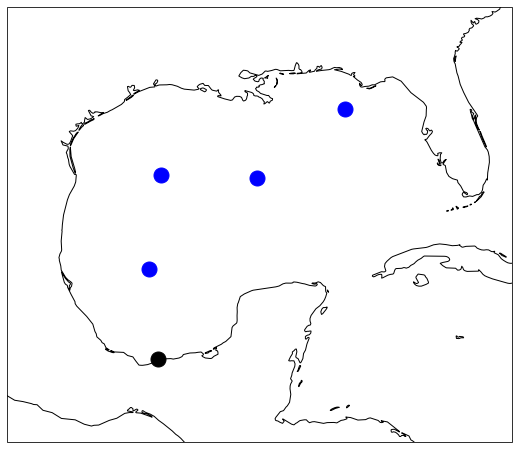
\includegraphics[width = .8\textwidth]{Figures/buoylocs}
\caption{Locations of buoys with observations of relevant wave variables. The buoy used in this project is marked in black, and other buoys are marked in blue}
\label{fig:buoylocs}
\end{figure}

As well as having limited observations, we also had limited access to forecast data, with only seven overlapping week-long forecast windows available. This raises questions over the robustness of the DA results, and so it would be useful for future studies to include more forecast data.

The lack of a forecast model will not be an issue in any future operational DA implmentation undertaken by Fugro. There are many ways in which the method used in this study could be modified to include cycling, and perhaps one of the simplest is to assimilate the observations as they are available in a more conventional ETKF setup. This would reduce the dimension of the state space since the state vector would only contain values from a single timestep. Observations could be assimilated every hour, or some observations could be skipped so that the DA could be performed less frequently to reduce computational cost. We have seen in this study that the ETKF reduces the ensemble spread in comparison to the forecast error, so this proposed method would be susceptible to filter divergence and some inflation or other preventative measure would likely be necessary to mitigate this.

Another possible approach would be to use a smoother method such as 4DEnVar. A smoother method simultaneously assimilates observations from an entire window, rather than assimilating observations from each observation time one by one as in a filter method. This would allow assimilation to be done less frequently while still assimilating all available obervations, and is less prone to filter divergence. However, this method would require the augmentation of the state vector to include values from multiple timesteps, and would require minimisation of the cost function using a method such as the conjugate gradient method \citep{Nocedal2006} which is typically computationally expensive. Further research should be done to determine the best approach. Schematics of both methods outlined here are shown in figure \ref{fig:altmethods}.

\begin{figure}
\centering
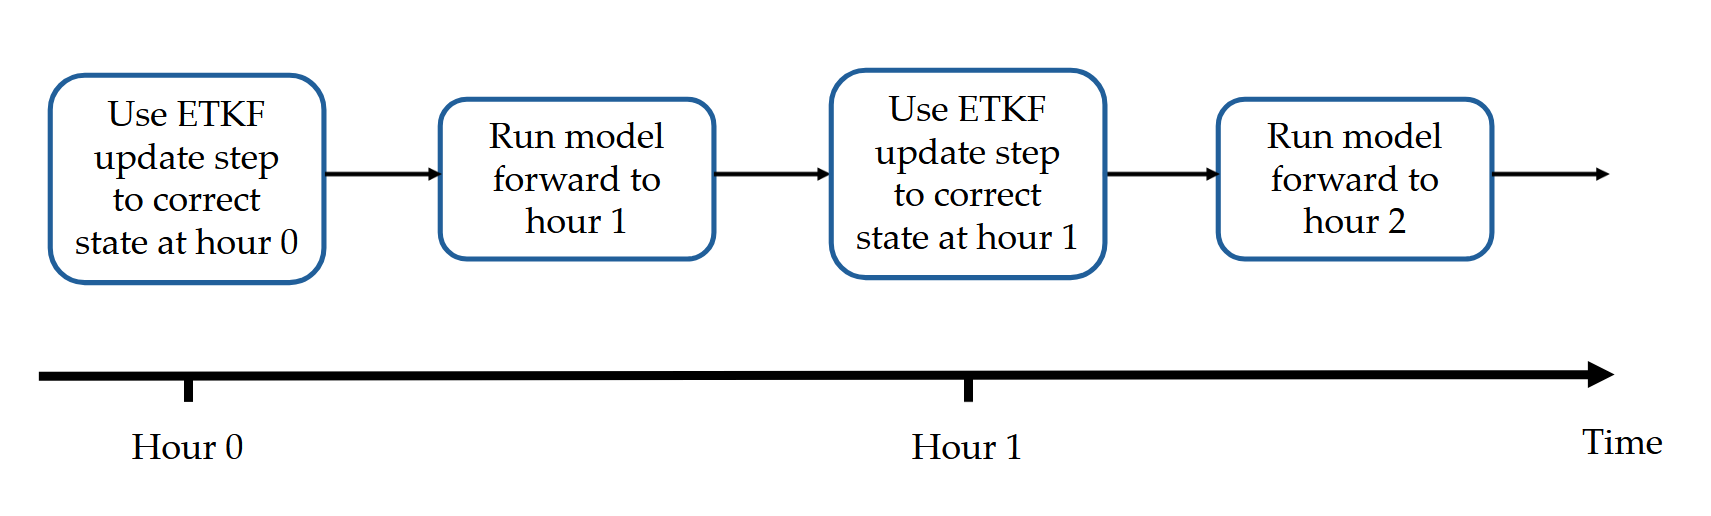
\includegraphics[width = \textwidth]{Figures/altfilter}
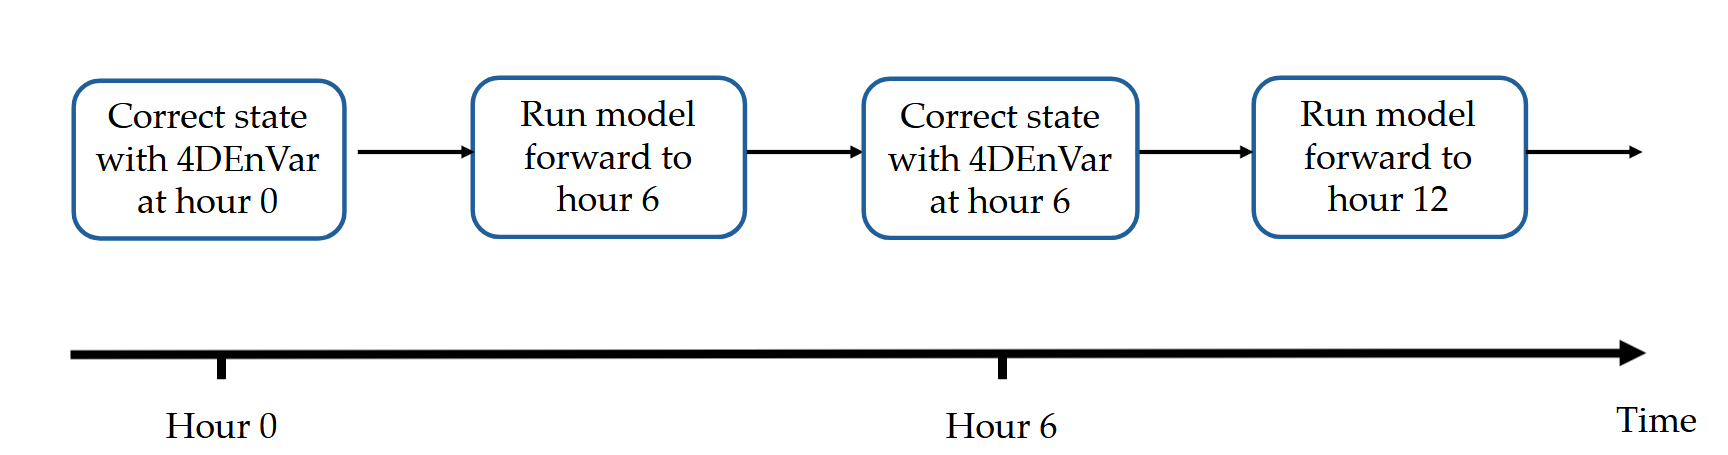
\includegraphics[width = \textwidth]{Figures/altsmoother}
\caption{Schematics of potential DA methods which incorporate cycling. Top: Observations assimilated hourly using a conventional ETKF filter method. Bottom: Observations assimilated every 6 hours using the 4DEnVar smoother method.}
\label{fig:altmethods}
\end{figure}

Since we have seen that the ensemble spread is reduced too much by the DA method used in this project, future studies into this topic chould include some kind of countermeasure against this effect. One possible countermeasure which has been discussed is inflation applied prior to the update step, which involves multiplying $\mat{P}^f$ by some predefined factor $\alpha >1$ before updating the model states. It is also possible to apply inflation during the analysis step by multiplying $\mat{P}^a$ by $\alpha$ prior to generating the analysis ensemble.

Other potential methods for artificially increasing the ensemble are adding noise to the forecast ensemble prior to calculating $\mat{P}^f$ \citep{Anderson1999}, or the method of relaxation from \cite{Whitaker2012}, in which the analysis ensemble is modified to bring it standard deviation closer to that of the forecast ensemble while leaving its mean unaffected.

Another problem encountered in this study is the large covariances and increments seen far away from the observation location. As discussed, this is often physically unrealistic, with spurious long distance covariances in $\mat{P}^f$ arising from sampling error and causing unrealistic large long-distance increments \citep{Hunt2007}. This may be improved with localisation, but since at least some of the long-distance covariances seen appeared to be genuine, we did not explore this in this study and left it instead for future work. Further investigation into the physical mechanisms behind the covariances would also be helpful here to inform the implementation of localisation.
